\documentclass[portuguese]{textolivre}

% metadata
\journalname{Texto Livre}
\thevolume{18}
%\thenumber{1} % old template
\theyear{2025}
\receiveddate{\DTMdisplaydate{2024}{7}{30}{-1}}
\accepteddate{\DTMdisplaydate{2024}{10}{16}{-1}}
\publisheddate{\DTMdisplaydate{2025}{1}{31}{-1}}
\corrauthor{Andrey Anderson dos Santos}
\articledoi{10.1590/1983-3652.2025.53776}
%\articleid{NNNN} % if the article ID is not the last 5 numbers of its DOI, provide it using \articleid{} commmand 
% list of available sesscions in the journal: articles, dossier, reports, essays, reviews, interviews, editorial
\articlesessionname{articles}
\runningauthor{Santos et al.}
%\editorname{Leonardo Araújo} % old template
\sectioneditorname{Daniervelin Pereira}
\layouteditorname{Leonardo Araújo}

\title{Estruturas de apoio às humanidades abertas}
\othertitle{Support structures for open humanities}

\author[1]{Andrey Anderson dos Santos~\orcid{0000-0001-8399-0035}\thanks{Email: \href{mailto:anndreys@gmail.com}{anndreys@gmail.com}}}
\author[1]{Edna Karina Lira~\orcid{0000-0001-5543-3792}\thanks{Email: \href{mailto:liraa.karina@gmail.com}{liraa.karina@gmail.com}}}
\author[1]{Eliana Maria dos Santos Bahia~\orcid{0000-0003-4037-3189}\thanks{Email: \href{mailto:eliana.maria@ufsc.br}{eliana.maria@ufsc.br}}}
\author[1]{Edgar Bisset Alvarez~\orcid{0000-0002-5388-5944}\thanks{Email: \href{mailto:edgar.bisset@ufsc.br}{edgar.bisset@ufsc.br}}}
\affil[1]{Universidade Federal de Santa Catarina, Programa de Pós-graduação em Ciência da Informação, Florianópolis, SC, Brasil.}

\addbibresource{article.bib}
\usepackage{array}

\begin{document}
\maketitle
\begin{polyabstract}
\begin{abstract}
Promover valores e princípios da Ciência Aberta facilita o acesso de acadêmicos e do público em geral aos resultados científicos em humanidades. No entanto, especialmente nessa área de conhecimento, observa-se uma relativa carência de entendimento sobre o papel crucial das práticas abertas de pesquisa que correspondem às expectativas sociais e econômicas contemporâneas. Destarte, suporte e orientação são ações essenciais para o desenvolvimento do discurso de abertura científica das humanidades. O objetivo do artigo é descrever elementos que ajudam a promover a Ciência Aberta por meio de estruturas de apoio às humanidades. Os objetivos específicos deste estudo são: descrever consórcios, associações e iniciativas do continente europeu que trazem suporte às humanidades; refletir sobre a comunicação desses elementos com a literatura sobre Ciência Aberta; e conscientizar sobre formas de manutenção e apoio às humanidades abertas. Esta investigação é um relato de experiência, que visa à identificação de: infraestruturas de pesquisa planejadas em longo prazo, suporte técnico para dados, centros de humanidades digitais, associações acadêmicas e redes de apoio, cujas contribuições sugerem possíveis aplicações para infraestruturas de humanidades em outros contextos.

\keywords{Humanidades abertas \sep Infraestrutura \sep Ciência aberta}
\end{abstract}

\begin{english}
\begin{abstract}
Promoting the values and principles of Open Science facilitates access for academics and the general public to scientific results in the humanities. However, in this particular field of knowledge, there is a noticeable lack of understanding regarding the crucial role of open research practices in meeting contemporary social and economic expectations. Therefore, support and guidance are essential actions for developing the discourse on scientific openness in the humanities. The aim of this paper is to describe elements that contribute to the promotion of Open Science through support structures for the humanities. The specific objectives of this study are: to describe consortia, associations, and initiatives across Europe that provide support to the humanities; to reflect on how these elements relate to the literature on Open Science; and to raise awareness about ways to sustain and support open humanities. This study is an experiential report that seeks to identify: long-term planned research infrastructures, technical support for data, digital humanities centers, academic associations, and support networks, whose contributions suggest possible applications for humanities infrastructures in other contexts.

\keywords{Open humanities \sep Infrastructure \sep Open science}
\end{abstract}
\end{english}
\end{polyabstract}

\section{Introdução}
A Ciência Aberta (CA) é retratada em conceitos, ferramentas e mídias que veiculam a comunicação e o compartilhamento da ciência em todo o processo de pesquisa, incluindo sua avaliação e disseminação \cite{picarra2016}.  Ela surgiu em decorrência do movimento em prol do Acesso Aberto às informações científicas e ao conhecimento. \textcite[p.~77]{saya2014} afirmam que a CA trouxe significados, dentre os quais o mais intenso é o que assume o conhecimento científico como “um patrimônio da humanidade e, que, portanto, deve estar disponível livremente para que as pessoas – cientistas ou não – possam usá-lo, reusá-lo e distribuí-lo sem constrangimentos tecnológicos, econômicos, sociais ou legais”.

A CA traz transparência para as pesquisas, bem como a possibilidade de seu compartilhamento e reutilização, fazendo com que elas sejam mais aprofundadas, gerem novos estudos e tragam desenvolvimentos por gerações \cite{pinheiro2019}. O movimento busca uma mudança sistêmica na forma como a ciência e a pesquisa têm sido tradicionalmente realizadas e compreende: Acesso Aberto aos resultados de pesquisa e infraestruturas de dados, desenvolvimento de novas habilidades, e reestruturação da carreira de pesquisadores – todos com o mesmo objetivo: uma ciência mais eficiente, melhor reproduzível e responsiva às expectativas sociais e econômicas \cite{european_commission2016}.

No campo das humanidades, encontramos imagens, vídeos e trabalhos interativos, por meio do engajamento entre as humanidades e a tecnologia da informação ou o digital \cite{svensson2010}. Dessa forma, cidadãos e acadêmicos conhecem e tornam conhecidos seus trabalhos científicos \cite{kamal2023}, os quais necessitam de uma extensa rede de apoio e de infraestruturas que favoreçam o contato de investigadores e da população em geral com os resultados desenvolvidos \cite{edmond2020}. Fora do sistema de publicação tradicional, repositórios digitais, softwares e páginas virtuais promovem o aprendizado e a pesquisa em humanidades por meio de conteúdos licenciados abertamente, que constituem uma relevante contribuição para a sociedade da informação.

Esses conteúdos transmitem os valores e princípios da CA, uma vez que os termos mais empregados ao descrevê-la são: “transparente”, “acessível”, “compartilhada” e “desenvolvida colaborativamente” \cite{vicente2018}. São os valores e princípios da CA que norteiam o debate sobre a ampliação do apoio às ciências humanas e sociais, de forma organizada e orientada à preservação digital de dados e informações necessárias nessas áreas de conhecimento. As humanidades abertas significam a intersecção entre as humanidades com as ferramentas próprias da CA na realização de uma ciência colaborativa e orientada à democratização dos seus conteúdos.

O termo “humanidades abertas” exige o desenvolvimento de um domínio comunicativo dedicado \cite{knockelmann2019open}. Encontra-se no continente europeu uma notória influência sobre o desenvolvimento de políticas que visam à abertura científica \cite{manco2022}, desde a sua taxonomia \cite{pontika2015} até as infraestruturas que a promovem \cite{kamocki2023,mounier2023}. Alguns desses componentes são centrais para a promoção das humanidades abertas. Refletir sobre alguns exemplos pode contribuir para as políticas brasileiras, aproveitando-se as notórias estruturas presentes no País, uma vez que no seu contexto geopolítico as iniciativas de Acesso Aberto estão presentes antes mesmo da fundação do conceito \cite{delrio2022}.

Esta pesquisa propõe-se a descrever os elementos que favorecem a CA na promoção da divulgação científica em humanidades. Os objetivos específicos deste estudo são: descrever consórcios, associações e iniciativas do continente europeu que trazem suporte às humanidades; refletir sobre a comunicação desses elementos com a literatura sobre CA; e conscientizar sobre formas de manutenção e apoio às humanidades abertas.

\section{Procedimentos metodológicos}\label{sec-normas}
Trata-se de relato de experiência, em que o período de vivências mais expressivo, de um ano, foi realizado durante o doutorado sanduíche junto à Universidade de Colônia, na Alemanha, especificamente no Centro de Colônia para Humanidades Digitais (CCeH). Esse contexto contribuiu para a percepção da intensidade do movimento em direção à publicação acadêmica em mídias, as quais ultrapassam o sistema científico tradicional, como \textcite{svensson2010} havia apontado que ocorreria gradualmente.

Tomando-se por partida o trabalho de \textcite{earnshaw2018}, verificaram-se iniciativas que possibilitam a publicação e a disseminação dos resultados de pesquisa em humanidades. Adicionalmente, identificaram-se outras estruturas locais, como laboratórios e centros científicos \cite{delrio2022}. Descrevemos a promoção das humanidades, bem como os princípios e valores da CA, por meio de documentos encontrados nos sites oficiais desses laboratórios ou centros. Também foi consultada a literatura desenvolvida por pesquisadores diretamente vinculados a eles. Os elementos de CA endereçados estão presentes na taxonomia elaborada por \textcite{silveira2021} (\Cref{fig1}) e nas práticas descritas por \textcite{morais2021}.

\begin{figure}
\centering
\begin{minipage}{\textwidth}
    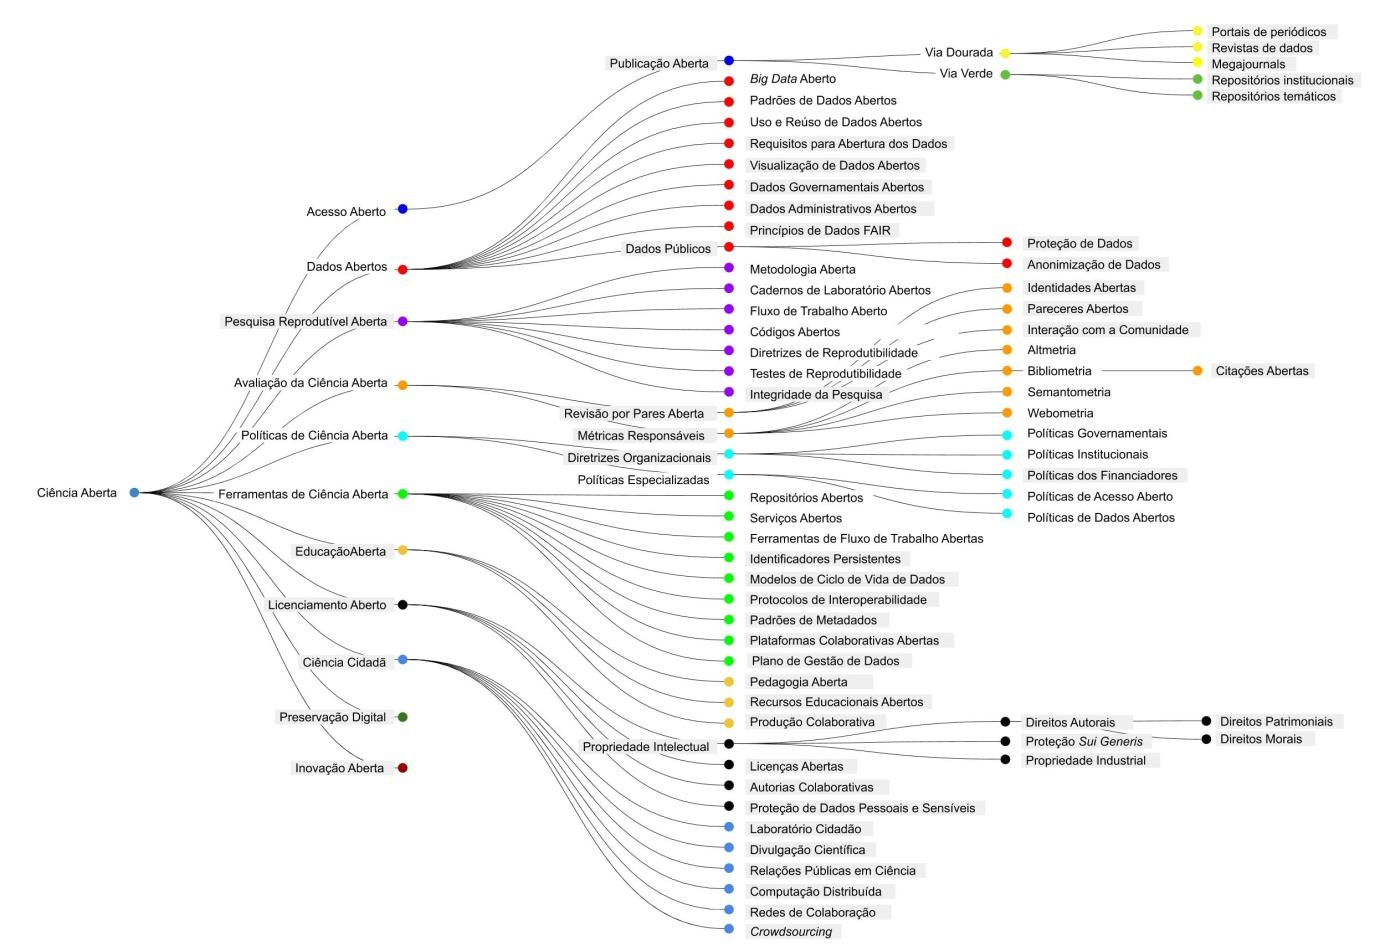
\includegraphics[width=\linewidth]{Fig1.png}
    \caption{Taxonomia da Ciência Aberta.}
    \label{fig1}
    \source{\textcite[p.~13]{silveira2021}}
\end{minipage}
\end{figure}

A seguir, serão apresentadas as estruturas de pesquisa em humanidades, por meio das quais se identifica a comunicação com elementos da literatura sobre CA. A discussão acerca dos fatores que promovem a taxonomia adotada é desenvolvida com mais profundidade na sétima seção do manuscrito e, na oitava seção, pode-se visualizar o que se pretende com o terceiro objetivo específico do estudo: conscientizar sobre formas de manutenção às humanidades abertas.

\section{Infraestruturas de pesquisa planejadas em longo prazo}\label{sec-conduta}
Uma das amplas preocupações da CA diz respeito a plataformas, ferramentas e serviços para disseminação e colaboração de conhecimentos \cite{fecher2013}. A partilha de recursos deve ser vista como um aspecto integral do trabalho com recursos digitais, abrangendo desde a criação e curadoria até a disseminação de recursos digitais para reutilização e aquisição de conhecimento – e não apenas como uma mera transferência de dados \cite{kalman2019}. Ao impactar quatro domínios interconectados (pesquisa, educação, cultura e economia), o consórcio DARIAH apoia o desenvolvimento sustentável e aberto da pesquisa digitalmente habilitada nas artes e humanidades, oferecendo ainda material didático e oportunidades de ensino para desenvolver habilidades de pesquisa digital \cite{dariah2024}.

DARIAH é um acrônimo para Infraestrutura de Pesquisa Digital para as Artes e Humanidades (em inglês: \textit{Digital Research Infrastructure for the Arts and Humanities}), que objetiva permitir a conexão entre pessoas, informações, ferramentas e metodologias para promover o uso de conteúdo digital em pesquisa, não apenas fornecendo tecnologia, mas facilitando a colaboração e o trabalho em diversas áreas das humanidades \cite{henrich2013}.

A participação em comunidades de pesquisa transnacionais, assim como o entendimento do impacto do patrimônio cultural digitalizado, são fundamentais para o avanço da pesquisa em humanidades com inovação e qualidade. A DARIAH promove a interação entre profissionais de patrimônio cultural, pesquisadores em humanidades e cientistas de dados, que muitas vezes se encontram limitados por desafios estruturais, legais e técnicos \cite{tasovac2020}.

A DARIAH possui uma forma jurídica própria, chamada de Consórcio Europeu para uma Infraestrutura de Investigação (\textit{European Research Infrastructure Consortium} – ERIC). O consórcio possibilita o estabelecimento em todos os países da União Europeia numa base não econômica, podendo realizar algumas atividades econômicas limitadas. Um ERIC conta com algumas isenções de impostos e pode adotar seus próprios procedimentos de contratação \cite{comissaoeuropeia2023eric}. Também se enquadram, nesse ordenamento, a Infraestrutura Comum de Recursos e Tecnologia da Linguagem (\textit{Common Language Resources and Technology Infrastructure} – CLARIN) e a Infraestrutura Europeia de Pesquisa sobre o Holocausto (\textit{European Holocaust Research Infrastructure} – EHRI), as quais promovem o uso eficiente de recursos, a viabilização de pesquisas multidisciplinares e o compartilhamento de boas práticas \cite{anuradha2024,bassett2019}.

\section{Suportes técnicos para dados}\label{sec-fmt-manuscrito}
As infraestruturas de pesquisa completam o seu sentido mais amplo se as instituições de educação e pesquisa também puderem atuar como centros de disseminação das competências para a CA – aqui, faz-se uma menção ao compartilhamento eficaz e, sobretudo, cauteloso de dados de pesquisa. A visibilidade e o impacto da pesquisa tendem a aumentar se os dados forem documentados e acessíveis, podendo ser utilizados por outros pesquisadores. De acordo com \textcite{stodden2009}, fornecer as fontes originais e o processo de coleta dos dados ou o código que gerou o conjunto de dados, bem como a enumeração de quaisquer alterações feitas no conjunto de dados, são ações essenciais para a reprodutibilidade da pesquisa.

Text+ é um consórcio projetado para atender todos os pesquisadores que trabalham com dados textuais e linguísticos, prestando apoio e aconselhamento individual. O suporte \textit{helpdesk} promovido por diversas instituições acadêmicas é oferecido em três domínios de dados – coleções, recursos lexicais e edições \cite{textplus2024}. Esses domínios exigem práticas de geração, curadoria e gerenciamento de dados distintas e interdisciplinares \cite{nfdi2024}.


\section{Centros de humanidades digitais}\label{sec-formato}
No nível de instituição universitária, as redes de apoio também são encontradas em centros de humanidades digitais. As humanidades digitais dizem respeito ao uso das tecnologias digitais nas ciências humanas \cite{adams2012} e ultrapassam a digitalização das suas disciplinas, uma vez que as tecnologias são igualmente empregadas para consecução de metodologias em ensino e pesquisa nas humanidades \cite{bailey2017}. Esse é um campo de pesquisa transdisciplinar, no qual as questões e objetos ligados às diversas disciplinas das ciências humanas, sociais e sociais aplicadas se unem aos recursos oriundos da computação, ocasionando a possibilidade de novos desdobramentos da produção do conhecimento nas humanidades no ambiente digital \cite{cuartas2017}. O relacionamento com a CA se deve à utilização das tecnologias para disponibilizar abertamente os processos de pesquisa, dados e resultados.

Os centros de humanidades digitais geralmente surgem a partir de um contexto de suporte de tecnologia da informação para acadêmicos, ou da união de diferentes projetos de pesquisa que formaram um centro, associados ou fisicamente localizados dentro das bibliotecas universitárias ou mesmo independentemente delas \cite{warwick2012}. Vinculados às bibliotecas, ressaltamos os propósitos de alguns desses centros:

\begin{enumerate}
    \item Biblioteca da Universidade Católica de Leuven, na Bélgica: oferece suporte a estudantes e alunos que pretendem adquirir ou melhorar as suas competências nas áreas de i) comunicação acadêmica e ciência aberta, ii) gestão de dados de pesquisa, e iii) ferramentas e métodos digitais \cite{budke2022}.
    \item Biblioteca da Universidade Carlos III de Madrid, na Espanha: pesquisadores em humanidades aproveitam a expertise da biblioteca, utilizando plataformas à disposição, ou explorando novos recursos e ferramentas num trabalho realizado conjuntamente entre bibliotecários e pesquisadores. O suporte é obtido tão somente se o conteúdo for disponibilizado em Acesso Aberto \cite{aguilera2021}.
    \item Biblioteca Nacional da França: a biblioteca projetou um laboratório voltado às humanidades digitais como um local de trabalho, intercâmbio e convivência para os pesquisadores. O espaço visa promover a experimentação e a Pesquisa e Desenvolvimento por meio de parcerias científicas, oferecendo uma gama de serviços presenciais e remotos para apoiar os seus usuários \cite{carlin2021}.
\end{enumerate}

Ademais, as bibliotecas contribuem para o armazenamento de objetos digitais e desempenham o relevante papel de promover o Acesso Aberto à pesquisa \cite{liu2023}. Uma das preocupações recorrentes diz respeito à preservação a longo termo desses conteúdos, por isso \textcite{zarnitz2019} descrevem um caso de cooperação entre bibliotecas da Alemanha, dado que a preservação digital demanda certa complexidade de processos e grande volume de recursos. Segundo os autores, os benefícios incluem a redução de custos, fluxos de trabalho e formatos de objetos digitais semelhantes, cooperação em atividades de rede e capacitação de pessoal. Desse modo, as bibliotecas contribuem para a expansão das humanidades, garantindo o acesso aos seus resultados e também a sua manutenção estrutural.


\section{Associações acadêmicas e redes de apoio}\label{sec-modelo}
O escasso financiamento das humanidades tende a ser de curto prazo, no máximo cinco anos. Todavia, requerem serviço profissional especializado e em tempo integral. Assim, os seus praticantes tendem a restringir-se à natureza de projetos, cujas metas também são de curto prazo, de modo que depois de encerrado o período de financiamento, praticamente não há meios para manter suas contribuições \cite{ghosh2015}.

Algumas iniciativas têm cooperado para o desenvolvimento permanente das humanidades não somente em sua agenda de pesquisa e ensino, mas também administrativa e política. Evidencia-se a criação de inúmeras associações, em que as aspirações nacionais ou regionais refletem práticas culturais e jurídicas próprias. As associações, em suas declarações estatutárias, permitem-nos enxergar os objetivos e as limitações de seus contextos, devendo funcionar em concordância com princípios democráticos que potencializem equidades dentro da ciência \cite{fiormonte2014}.

A Associação Europeia para as Humanidades Digitais (\textit{European Association for Digital Humanities} – EADH), fundada em 1973, é a mais antiga e hoje a maior organização de humanidades digitais. A associação possui algumas revistas, a \textit{Digital Scholarship in the Humanities} (DSH), a \textit{Digital Humanities Quarterly} (DHQ) e a \textit{Digital Studies / Le champ numérique}. A EADH é um membro fundador da Aliança Internacional de Organizações de Humanidades Digitais (\textit{Alliance of Digital Humanities Organizations} – ADHO), que serve à comunidade científica internacional promovendo prêmios, conferências e publicações \cite{eadh2024}.

A ADHO promove a investigação e o ensino com abrangência intercontinental, incluindo países como Canadá, África do Sul, Japão, México, entre outros. Os seus membros provêm de diversos departamentos acadêmicos, como Inglês, Francês, Línguas Modernas, Linguística, História, Filosofia, Teatro, Música, Ciência da Computação e Artes Visuais. Os objetivos da associação são: i) apoiar e promover a pesquisa e a educação em humanidades digitais; ii) servir como uma força consultiva baseada na comunidade para as humanidades digitais; iii) incentivar a excelência na pesquisa, publicação, parceria e educação em humanidades digitais \cite{adho2024}.

A conferência anual da ADHO é de relevância central para as humanidades. O evento reúne pesquisadores de diversas partes do mundo, mas ressalta-se que o seu escopo ainda carece de práticas inclusivas, orientadas a culturas e necessidades que não compõem o contexto anglo-americano \cite{estill2022,mahony2018}. Considerando que os trabalhos apresentados na conferência anual são referência para o campo científico \cite{du2019}, é fundamental promover a inclusão de diversas perspectivas para evoluirmos acadêmica e socialmente, fazendo jus aos atributos de abertura, colaboração e colegialidade \cite{poole2017}.

A Rede de Métodos Digitais nas Artes e Humanidades (\textit{Network for Digital Methods in the Arts and Humanities} – NeDiMAH), a Humanidades no Espaço Europeu da Investigação (\textit{Humanities in the European Research Area} – HERA) e o Conselho de Pesquisa em Artes e Humanidades (\textit{Arts and Humanities Research Council} – AHRC) contribuíram e contribuem para um indelével legado para a pesquisa e ensino em humanidades \cite{earnshaw2018}.

A rede NeDiMAH proporcionou a classificação e a expressão das artes e humanidades digitais com foco em três principais resultados: um mapa de visualização do uso da pesquisa digital em toda a Europa; um fórum online para praticantes ativos na área; e uma ontologia de métodos de pesquisa digital \cite{european_science_foundation2012}. A ontologia desenvolvida é estruturada em uma camada superior com conceitos gerais, uma intermediária com detalhes aplicáveis a todos os domínios das humanidades, e uma camada inferior que, por meio de relações de especialização de classe e propriedade e de vocabulários hierárquicos controlados, captura os pormenores de domínios e assuntos \cite{pertsas2017}.

A HERA é uma rede multilateral criada em 2004 para promover e apoiar a pesquisa em humanidades na Europa. Além de compartilhar a excelência nas práticas e resultados de gestão de pesquisa, busca desenvolver oportunidades de financiamento a pesquisadores. Para isso, os 25 países europeus atualmente membros contam com o apoio de 26 organizações de financiamento parceiras da rede \cite{hera2023}.

O AHRC financia pesquisas e estudantes do Reino Unido em mais de 50 disciplinas – desde história, artes cênicas, linguagem, filosofia, museologia, literatura, religião e design, até as menos convencionais, como \textit{big data}, saúde, meio ambiente e bem-estar, a fim integrar as artes e humanidades com outras disciplinas \cite{ahrc2018}. Considerando o papel da literacia digital para gerir, arquivar e manter recursos de forma sustentável e acessível, bem como a necessidade de aperfeiçoamento dos pesquisadores em humanidades nessas atividades, o AHRC executou algumas ações. Entre elas, a produção de uma nova política especificando requisitos relativos à criação, armazenamento e compartilhamento de dados e software em artes e humanidades; o incentivo a treinamentos de pesquisadores; e a atualização do guia de financiamento de pesquisa, esclarecendo o apoio a especialistas em dados, como engenheiros de software de pesquisa \cite{siewicz2022}.

\section{Elementos de Ciência Aberta presentes nas iniciativas retratadas}\label{sec-organizacao}
Os dados produzidos em pesquisa englobam uma variedade de informações, arquivos e registros que são produzidos ou utilizados para demonstrar e validar os resultados em investigações \cite{comissaoeuropeia2017}. No contexto dos dados abertos, a adoção dos princípios FAIR (\textit{Findable, Accessible, Interoperable, Reusable}) (\Cref{tab01}) é fundamental para facilitar a reutilização contínua dos dados em diversas implementações \cite{wilkinson2016}.

\begin{table}[h!]
\centering
\begin{threeparttable}
\caption{Princípios FAIR.}
\label{tab01}
\begin{tabular}{>{\raggedright\arraybackslash}p{3cm} >{\raggedright\arraybackslash}p{11cm}}
\toprule
Princípio & Descrição \\
\midrule
\textit{Findable} (Localizável) &  Visa à descoberta de dados por humanos e sistemas de computador.  \\
\textit{Accessible} (Acessível) & Diz respeito a como acessar os dados, possivelmente incluindo autenticação e autorização. \\
\textit{Interoperable} (Interoperável) & Significa que os dados podem ser integrados com outros dados. \\
\textit{Reusable} (Reusável) & Especificando as licenças de uso, aumenta-se a reutilização de dados. \\
\bottomrule
\end{tabular}
\source{adaptado de \textcite{brinkman2023}.}
\end{threeparttable}
\end{table}


O princípio \textit{Findable} (Encontrável) de dados abertos também se baseia na capacidade de um objeto ser acionável, mesmo que não exista mais o responsável pela atribuição de um link. Um ORCID iD é um exemplo de identificador persistente para uma pessoa, enquanto os DOIs (\textit{Digital Object Identifiers}, ou Identificadores de Objetos Digitais) são identificadores persistentes para coisas ou entidades, como artigos de periódicos, livros e conjuntos de dados, cujos principais atribuidores são Crossref e DataCite \cite{orcid2023}.

A abertura dos dados tem o potencial de minimizar a duplicação de esforços e, consequentemente, acelerar o progresso em questões críticas para a ciência \cite{clark2021}. A DARIAH desempenha um papel crucial na promoção dos dados abertos, pois reconhece a relevância de disponibilizar conjuntos de dados relacionados ao patrimônio cultural em formatos que atendam aos princípios FAIR \cite{tasovac2020}.

O Repositório DARIAH-DE compreende um arquivo digital de longo prazo para dados de pesquisa em humanidades e ciências culturais. Toda a preparação para publicação envolve três etapas: primeiro, é necessário criar uma coleção; segundo, todos os dados associados à coleção são carregados e, finalmente, todos os dados são descritos por metadados. O padrão de metadados utilizado é o Dublin Core Simple e apenas alguns campos são obrigatórios, como informações de licença. Além disso, identificadores persistentes para referência estável são fornecidos: as coleções e todos os objetos associados recebem Identificadores Digitais de Objetos (DOIs) individuais. Uma vez publicados, todos os dados estão publicamente disponíveis \cite{kalman2019}.

Complementando a abordagem centrada em dados e considerando a sensibilidade em compartilhar aqueles dados provenientes dos povos indígenas, surgiram os princípios CARE (\textit{Collective Benefit, Authority to Control, Responsibility, and Ethics}). Essa sigla compõe um significado emblemático ao ser empregada na expressão “Be FARE and be CARE!”, podendo ser traduzida do inglês como: “Seja justo e tenha cuidado!”. \textcite{carroll2020} assim descrevem os princípios:

\begin{enumerate}
    \item \textit{\textbf{Collective Benefit}} \textbf{(benefício coletivo)}: os dados precisam beneficiar o coletivo a fim de alcançar desenvolvimento e inovação inclusivos, melhorar a governança e o envolvimento do cidadão e obter resultados equitativos.
    \item \textit{\textbf{Authority to Control}} \textbf{(autoridade para controlar)}: esse princípio reforça a autoridade dos povos para controlar e governar seus dados e determinar os protocolos de governança, enquanto estão ativamente envolvidos nas decisões de administração quando os dados são mantidos por outras entidades.
    \item \textit{\textbf{Responsibility}} \textbf{(responsabilidade)}: exige-se responsabilidade em cultivar relacionamentos respeitosos com os povos de quem os dados se originam. A responsabilidade final consiste em apoiar os dados que promovem a autodeterminação e o benefício coletivo.
    \item \textit{\textbf{Ethics}} \textbf{(ética)}: é fundamental a representação e participação dos povos, que podem avaliar os benefícios, danos e possíveis usos futuros de seus dados, com base na ética da comunidade.
\end{enumerate}

O conjunto de práticas que envolve o uso eficaz e cauteloso de dados muitas vezes carece de uma compreensão precisa quanto aos seus propósitos. Especialmente nas humanidades, falta entendimento acerca do papel crucial que os dados desempenham \cite{learn2017,taylor2022}. Portanto, suporte e orientação são ações essenciais para o desenvolvimento de uma pesquisa reprodutível aberta.

O consórcio Text+ fornece orientação em todas as fases do ciclo de vida dos dados: execução de princípios FAIR e CARE, bem como Planos de Gestão de Dados (PGD) para novos projetos de pesquisa. A relação entre CA e PGD é o armazenamento e a preservação de dados de pesquisa, a fim de garantir tanto a integridade da pesquisa quanto a reutilização dos dados preservados \cite{botevericad2022}. Por meio de diretrizes estruturadas, busca-se garantir que os dados de pesquisa sejam rastreáveis, disponíveis, autênticos, citáveis, armazenados adequadamente e que cumpram parâmetros legais e de segurança que regem o uso subsequente \cite{learn2017}.

A CA também aborda o processo científico fundamentado no trabalho cooperativo e em formas de disseminar o conhecimento, melhorando a acessibilidade e a reutilização dos resultados da investigação a partir da utilização das tecnologias digitais e ferramentas colaborativas \cite{morais2021}. As associações e redes de apoio contribuem para o fazer científico aberto, seja funcionando como um elo para que os pesquisadores compartilhem seus resultados e colaborem entre si, seja apoiando a realização de pesquisas digitalmente habilitadas, cujas ferramentas aproximam-se dos parâmetros de construção colaborativa e interdisciplinar da CA. Ademais, elas editoram periódicos de Acesso Aberto e adotam políticas de CA ao financiar projetos de pesquisa cujos resultados devem ser publicados em Acesso Aberto, o que permite a reprodução e a disseminação científica dos seus trabalhos.

Na literatura, as bibliotecas se destacam como um referencial na elaboração de materiais de consulta quando uma determinada política de Acesso Aberto é implantada numa instituição de pesquisa \cite{liu2023}. Por meio da inserção dessas e outras atividades no cotidiano do bibliotecário, essas instituições vêm afirmando novos papéis \cite{cryer2011}, até mesmo quando as políticas de Acesso Aberto não estão oficialmente implantadas \cite{harrington2022}. Isso vai ao encontro dos achados, uma vez que os centros de humanidades instalados fisicamente nessas instituições contam com a expertise na disponibilização de conhecimento em Acesso Aberto e um ambiente que favorece o contato e a colaboração científica entre pesquisadores. Além disso, as bibliotecas atuam na preservação digital de conhecimento em longo prazo \cite{anyaoku2019}. Essa e outras práticas presentes nas experiências retratadas são sintetizadas na \Cref{tab02}.

\begin{table}[h!]
\centering
\begin{threeparttable}
\caption{Elementos da Ciência Aberta promovidos por estruturas de Humanidades no continente.}
\label{tab02}
\begin{tabular}{>{\raggedright\arraybackslash}p{3cm} >{\raggedright\arraybackslash}p{5.2cm} >{\raggedright\arraybackslash}p{5.2cm}}
\toprule
Estruturas & Exemplos & Elementos de Ciência Aberta \\
\midrule
Infraestruturas de pesquisa planejadas a longo prazo & Infraestrutura de Pesquisa Digital para as Artes e Humanidades (DARIAH)

Infraestrutura Comum de Recursos e Tecnologia da Linguagem (CLARIN)

Infraestrutura Europeia de Pesquisa sobre o Holocausto (EHRI) & Colaboração interdisciplinar

Dados abertos

Identificadores persistentes

Preservação digital

Repositórios Digitais abertos \\
Suporte técnico para dados & Text+ & 
Dados abertos

Plano de Gestão de Dados \\
Centros de humanidades digitais & Biblioteca Nacional da França

Biblioteca da Universidade Carlos III de Madrid

Biblioteca da Universidade Católica de Leuven & Acesso Aberto

Capacitação em Ciência Aberta

Colaboração interdisciplinar

Preservação digital \\
Associações acadêmicas e redes de apoio & Associação Europeia para as Humanidades Digitais (EADH)
Aliança Internacional de Organizações de Humanidades Digitais (ADHO)

Rede de Métodos Digitais nas Artes e Humanidades (NeDiMAH)

Humanidades no Espaço Europeu da Investigação (HERA)

Conselho de Pesquisa em Artes e Humanidades (AHRC) & Acesso Aberto

Colaboração interdisciplinar

Pesquisa Reprodutível Aberta \\
\bottomrule
\end{tabular}
\source{elaborado pelos autores (2024).}
\end{threeparttable}
\end{table}

Entende-se que os elementos mencionados não exaurem todas as possibilidades perceptíveis em suas estruturas, afinal a análise de outras interações políticas e científicas nelas presentes exigiria outras técnicas de levantamento de dados para a nossa pesquisa. Essas estruturas nos permitem, porém, induzir com acerto a existência de uma vertente lógica para a abertura científica nas humanidades. Adicionalmente, as formas como estão organizadas e estabelecidas nos fornecem algumas pistas sobre como manter e apoiar as humanidades abertas, como se verá adiante.

\section{Formas de manutenção e apoio às humanidades abertas}\label{sec-organizacao-latex}
Assim como em outras áreas do conhecimento, é necessário abrir os projetos fechados em silos, que acabam por produzir e reproduzir dados incompreensíveis. Salienta-se que focar no uso de recursos digitais é fundamental. Ao fazer pesquisas digitalmente habilitadas, criam-se melhores condições de utilizar e compartilhar as coleções digitais de acesso gratuito, aproveitando-se de uma infraestrutura de investigação que realiza verdadeiras transformações \cite{ell2013}.

Percebe-se a necessidade de coexistirem redes de apoio para a aplicação das técnicas digitais na investigação em humanidades e para a disseminação das competências em CA. Uma infraestrutura de acesso ao conhecimento deve ainda prover conteúdos produzidos em outras línguas e regiões \cite{mounier2023}, considerando novas formas e mídias para comunicação da ciência. Um modelo estrutural para avanço na temática requer, portanto, a integração entre infraestruturas e parcerias que perpassam disciplinas, espaços geográficos e sistemas de recompensa profissionais.

Demanda-se a instituição de setores próprios para o gerenciamento da CA. Enquanto há serviços em universidades e instituições de pesquisa que estão dispersos, a unificação de estratégias pode proporcionar funcionalidades mais coesas e assertivas em prol do acesso ao conhecimento. Uma agência para CA formada por uma equipe interdisciplinar é essencial para gerir as questões complexas da ciência, combinando perspectivas plurais na promoção da pesquisa em humanidades e em outras áreas \cite{ribeiro2024}.

Conforme \textcite{kamal2023}, as infraestruturas de investigação são mediadoras entre as exceções legais para reutilização do conhecimento e os requisitos da CA. Por consequência, todo o desenvolvimento das estruturas aqui tratadas implica a descentralização do conhecimento fazendo uso de licenças abertas. O cenário é prospectivo a esses conteúdos, uma vez que os agentes financiadores têm assumido um papel crucial ao exigir que as pesquisas patrocinadas estejam disponíveis em Acesso Aberto \cite{else2021}.

A compreensão sobre sustentabilidade no contexto abordado atualmente baseia-se no seguinte modelo mental: uma vez concluído, é relativamente estável e, dentro das expectativas normais para as condições ambientais, provavelmente estará disponível e poderá ser descoberto por meio de uma biblioteca para longo prazo. Todavia, a manutenção do conhecimento gerado não obedece a regras simplistas como essas e continua a ser um desafio constante no ecossistema mais amplo das humanidades digitais \cite{edmond2020}.

Afinal, o crescente volume de dados do patrimônio cultural e de material digital gerado – como resultado de dados de pesquisas, análises de materiais, arte digital, bibliografias e demandas contemporâneas – torna prioritário gerir uma grande quantidade de dados, disponibilizando-os numa dimensão regional e global \cite{fresa2013}. Isso torna desafiador o andamento de organizações de apoio à pesquisa e preservação digital. Justifica-se, assim, a criação de estruturas de armazenamento de dados de pesquisa e a contratação de pessoas para geri-los \cite{ahmad2022,cordeiro2018}, tendo em vista a demanda por estabelecimento de políticas internas, ordenamento jurídico condizente com a dinâmica científica, além de sustentabilidade financeira.

Após a estruturação interna dessas organizações, \textcite{risslerpipka2023} ratificam que externamente o desafio é conectar todas as estratégias e ofertas de serviços de investigação e de dados entre os níveis nacional e internacional. Nada se resolve pela tecnologia em si, mas a partir de políticas que precisam ser tratadas institucional e interdisciplinarmente \cite{luz2018}.

Com base nos resultados apresentados, ressalta-se que um modelo estrutural para humanidades abertas tem que considerar os desafios inerentes à temática, dentre eles: literacia digital, práticas de pesquisa responsáveis, multilinguismo e preservação digital. As subestruturas devem estar atentas à constituição de quaisquer planos nacionais e internacionais para financiá-las, pois os recursos são historicamente escassos. Uma vez que a integração é a palavra de ordem, a abordagem unificada e colaborativa para avançar no campo das humanidades deve ser idealmente seguida, requerendo ainda instituição de associações e organizações que prezem pela equidade de seus membros.

\section{Considerações finais}\label{sec-autores}
Ao passo que a ciência tradicional clama por uma mudança de paradigma editorial, as humanidades abertas naturalizam a ocorrência de transformações, com estruturas de apoio que sustentam as aplicações tecnológicas e a abertura das suas produções. Os consórcios, associações e iniciativas descritos neste artigo permitem vislumbrar novas formas de comunicação e disseminação científica. Por meio dessas estruturas, a dinâmica das humanidades evidenciou os seguintes aspectos: Acesso Aberto, Dados Abertos, Repositórios Digitais Abertos, Identificadores Persistentes, Preservação Digital, Plano de Gestão de Dados de Pesquisa e Colaboração Interdisciplinar.

Naturalmente, em todo o mundo há instituições e organismos que promovem esses aspectos. A pesquisa não pretende esboçar um modelo de humanidades abertas estritamente com base em experiências de outros contextos geopolíticos, uma vez que o Brasil e a América Latina possuem estruturas próprias e até pioneiras no campo. As infraestruturas descritas e que se estabelecem como consórcios recebem destaque no texto pela sustentabilidade financeira e pelo planejamento em longo prazo. A ênfase da investigação está voltada à democratização da ciência, que é tanto um corpo de conhecimento quanto um processo que visa à sua disseminação.

Para o cenário nacional, a principal reflexão é que uma infraestrutura de humanidades abertas demanda criações estáveis e integradas. Não se concretiza a partir de uma rígida entidade jurídica, mas de eixos funcionais que viabilizam: publicação científica em diferentes mídias e formatos, produção de recursos educacionais multilíngues, suporte e financiamento para o compartilhamento e preservação de dados de pesquisa. A partir desses fatores, a área de humanidades fortalece o uso de seus conteúdos na pesquisa e no ensino. As experiências brasileiras concretizam seus avanços, mas o que fica de lição é como encurtar o distanciamento entre as estruturas existentes e os pesquisadores, cujo contato com a sociedade pode estar limitado aos projetos de curta duração, à fragmentação entre disciplinas, ou à insipiência das práticas de abertura científica, que são desafios a serem superados também em outras áreas de conhecimento.

Há uma história marcada por iniciativas que apoiam as humanidades e as estabelecem administrativa e politicamente, por meio de associações, redes de apoio e bibliotecas. As estratégias coletivamente elaboradas nesses contextos têm que ser priorizadas. É necessário um diálogo nacional constante entre essas estruturas para humanidades, de forma que sejam integradas desde a sua concepção, possibilitando um melhor aproveitamento de recursos e fazendo valer a máxima em que o todo é maior que a soma das partes.

\section{Agradecimentos}\label{sec-idioma}
O presente trabalho foi realizado com apoio da Coordenação de Aperfeiçoamento de Pessoal de Nível Superior – Brasil (CAPES) – Código de Financiamento 001. Os autores agradecem a avaliação por pares e a revisão linguística deste manuscrito, cujas contribuições aprimoraram a qualidade do texto e a clareza na apresentação do conteúdo.



\printbibliography\label{sec-bib}
%conceptualization,datacuration,formalanalysis,funding,investigation,methodology,projadm,resources,software,supervision,validation,visualization,writing,review
\begin{contributors}[sec-contributors]
\authorcontribution{Andrey Anderson dos Santos}[conceptualization,investigation,methodology,funding,writing]
\authorcontribution{Edna Karina Lira}[methodology,writing,review]
\authorcontribution{Eliana Maria dos Santos Bahia}[writing,review]
\authorcontribution{Edgar Bisset Alvarez}[conceptualization,methodology]
\end{contributors}
\end{document}
